

\chapter{Classical Groups}\label{chap2}%chapterII

Throughout\pageoriginale the rest of these lectures we shall assume the
characteristic of the ground field $K$ to be zero. In the first three
paragraphs of this chapter we collect the basic facts on semi-simple
linear algebraic groups (basic references \cite{keyC3}, \cite{keyD-G}). The last
three paragraphs contain a survey of classical groups
(\cite{keyDi}, \cite{keyW2}). 



\section{Linear algebraic groups}\label{chap2:sec2.1}

By a linear algebraic group $G$ over $K$ we mean an affine algebraic
variety $G$ defined over $K$ together with $K$-morphisms $G \times G
\rightarrow G$ denoted by $(x,y) \rightarrow x.y$ and $G \rightarrow
G$ denoted by $x \rightarrow x^{-1}$ which satisfy the group
axioms. Whenever we talk of  open or closed sets in a variety we
shall always assume that they are so in the Zariski topology. For any
field of definition $L$ the group of points of $G$ rational over $L$
will be denoted by $G_{L}$. 

\begin{example*}
$G = GL_n$ the general linear group; if $\Omega$ is the universal
  domain over $K$ this is the algebraic group $GL_n(\Omega)$ of
  non-singular $n \times n$ matrices with entries in $\Omega$. If $x
  = (x_{ij}) \in GL_n (\Omega)$ the mapping  $(x_{ij}) \rightarrow
  (x_{11},x_{12}, \ldots , \ldots x_{n n},(\det x)^{-1})$ gives an imbedding of
  $G$ in $\Omega^{n^2+1}$ as  a closed subvariety of  $\Omega^{n^2+1}$,
  $GL_n$ is an algebraic group defined over the prime field and for any
  field $L$, $(GL_n)_{L} = GL_n (L)$.  
\end{example*}

\noindent
Next\pageoriginale if $\mathscr{G}$ is a non-degenerate quadratic form
over $K$ its 
orthogonal group $0 (\mathscr{G})$ is a closed subgroup of $GL_n$ and
is an algebraic group defined over $K$. It is known that any linear
algebraic group is isomorphic (i.e biregular isomorphism) to an
algebraic (i.e. closed) subgroup of $GL_n$  for some $n$. The
connected component of the  identity of the algebraic group $G$ is
denoted by $G_\circ ; G_o$ is a closed, normal and connected  subgroup of
$G$ with $[G:G_\circ] < \infty $; conversely any closed normal and
connected subgroup of $G$ of finite index must be $G_\circ$. In the
example above the connected component of the identity of $0 (
\mathscr{G} )$ is $ S \circ (\mathscr{G}) $ the special orthogonal group
of $\mathscr{G}$ i.e. the subgroup of elements of $0(\mathscr{G})$
with determinant $1; S 0 ( \mathscr{G}) $ is of index two in $0
(\mathscr{G})$. For any linear algebraic group $G$ there exists a
unique  maximal normal, connected and solvable subgroup $G_1$, called
the radical of $G$. We make the following 

\begin{defn}\label{chap1:def1}%def 1
A linear algebraic group $G$ is said to be semi-simple if its radical
$G_1 = \{1\}$. 
\end{defn}

\setcounter{exam}{1}
\begin{exam}%% 2
  It is known that $SL_n$. the subgroup of elements of $GL_n$ with
  determinant 1 is a semi-simple algebraic group. 
\end{exam}

\begin{exam}%% 3
The orthogonal group $0 (\mathscr{G})$ of a non-degenerate quadratic
form in at least three variables is semi-simple. 
\end{exam}

Let $H$ be a connected linear algebraic group defined over $K$. Then
we have the following  

\begin{defn}%def 2
$A$ covering of $H$ is a pair $(G,f)$, where $G$ is a
  connected\pageoriginale linear algebraic group and  $f:G
  \rightarrow H$ is a homomorphism (i.e. rational homomorphism)
  which is surjective and with finite kernel, (for the definition of
  surjectivity, exactness etc, see \ref{chap1:sec1.6}); 
\end{defn}

\begin{defi*}%def 
A linear algebraic group $G$ is said to be simply connected if it is
connected and every covering of it is an isomorphism. 
\end{defi*}

\begin{rem}\label{chap2:rem1}
In the case of  non-zero characteristic $p$, this definition is not
reasonable; $SL_n$ would not be simply connected in the above
definition because $(x_{ij}) \rightarrow (x^{p}_{ij})$ is surjective
with finite kernel but is not  an isomorphism. But $SL_n$ is simply
connected in the above definition if the characteristic is zero. 
\end{rem}

\begin{rem}\label{chap2:rem2}
If $(G,f)$ is a covering of the connected  linear algebraic group $H$
then $ker f \subset $ center $G$; for let $N = \ker f$: then $N$ is a
finite group and so the Zariski topology on $N$ is discrete. For every
$n \in N$ consider the morphism  $G \rightarrow N$ given by $x
\rightarrow x n x^{-1}n^{-1}$; since $G$ is connected and $N$ discrete
this must be a constant map; taking $x = n$, this constant value must
be 1; i.e. $xnx^{-1} n^{-1} = 1 \forall x \in G$; since $n \in N$ 
 may be quite arbitrary $N$ must be in the center of $G$.  
\end{rem}

\begin{defi*}%def
A linear algebraic group $G$ is said to be simple if its only closed
normal subgroups are the identity and $G$ itself. 
\end{defi*}

\begin{example*}
The projective linear group $PGL_n$ which is the quotient of $GL_n$ by
its center is a simple group.  
\end{example*}


\section{Semi-simple groups}\label{chap2:sec2.2}

If $G$ is any linear algebraic group the adjoint group  $\bar{G}$ is
defined to be the quotient of $G$ by its centre. It is known that a
semi-simple\pageoriginale linear algebraic group has finite center. If
$G$ is a 
connected semi-simple linear algebraic group defined over $K$ there
exists a covering  $\tilde{G} \rightarrow G $ defined over $K$ such
that $\tilde{G}$ is simply connected and that $\tilde{G}$ is unique
upto $K$-isomorphism; $\tilde{G}$ is called the universal covering
group of $G$. 

\setcounter{exam}{0}
\begin{exam}\label{chap2:exam1}%% 1
The adjoint group of $SL_n$ is the projective linear group $PGL_n$. 
\end{exam}

\begin{exam}\label{chap2:exam2}%% 2
Let $\mathscr{G}$  be a non-degenerate quadratic form on a finite
dimensional $K$-vector space $V$. The proper orthogonal group $S0
(\mathscr{G})$ is semi-simple and connected; and it has a two fold
covering namely the Spin group which is constructed using the Clifford
algebra of $\mathscr{G}$; we merely state the definition and
properties of Clifford  algebra and refer the reader to the standard
works  \cite{keyB}  Chap. 9 and \cite{keyC1}. A Clifford algebra of
$\mathscr{G}$ 
is a pair $(C,f)$ where $C$ is an associative $K$-algebra with
unity and $f:V \rightarrow C$ is a $K$-linear map with $\{f (x)\}^2 =
q (x) \cdot 1$ for every  $x \in V$ and satisfying the following universal
property: Whenever a pair $(D,g)$ is given with $D$ an associative
$K$-algebra with unity and  $g:V \rightarrow D$ is a $K$-linear map such
that $\{g(x)\}^2 =\mathscr{G} (x).1$ there exists a unique $K$-algebra
homomorphism $h: C \rightarrow D$ making the diagram 
\[
\xymatrix{
V \ar[rr]^f \ar[dr]_g & & C \ar[dl]^h \\
& D & 
}
\]
commutative.\pageoriginale It is known that such an algebra $C$ exists
and is unique upto $K$-isomorphism; evidently $f(V)$ must generate
$C$. The algebra $C$ is called the Clifford algebra of $\mathscr{G}$
and is denoted by $C (\mathscr{G})$. It turns out that the map $f$ is
injective, so we can identify $f(V)$ with $V$; then if $e_1,\ldots,
e_n$ is a basis of 
$V$, the products $e_{i_{1}} \ldots e_{i_{m}} (1 \leq i_1 < i_2 <
\ldots < i_m \leq n, 1 \leq m \leq n)$ together with 1 form a basis
of $C(\mathscr{G})$ so its dimension is $2^n$. If $n$ is even $C$ a
simple algebra  with centre $K$; if $n$ is odd the algebra $C$ is a
separable algebra, its centre being of dimension two over $K$; $C$ is
either simple or the direct sum of two simple algebras. We denote by
$C^+$ the subalgebra of $C$ generated by products of an even number
of vectors of $V$; then $\dim C^+ = 2^{n-1}$.  
\end{exam}

In case $n = \dim V $ is even and $n>0$ it is known that $C^+
(\mathscr{G})$ is separable its centre $Z$ is of dimension 2 over
$K$; $Z$ is either a quadratic extension of $K$ or a direct sum of two
copies  of $K$; in the first case $C^+ (\mathscr{G})$ is a simple
algebra while in the second case it is a direct sum of two simple
algebras. If $n$ is odd then $C^+ (\mathscr{G})$ is  always central
simple; if in  addition $\mathscr{G}$ has maximal Witt index then $
C^+ (\mathscr{G})$  is isomorphic to the ring $M_{\dfrac{n-1}{2}} (K)$,
of  $\dfrac{n-1}{2} \times \dfrac{n-1}{2}$ matrices over $K$. If $L$ is
any extension of $K$ then the quadratic form $\mathscr{G}$ can be
extended to a quadratic form $\mathscr{G}_{L}$ of $V_{L}$ in a natural
way by passing to the associated bilinear form of $\mathscr{G}$ and
extending it to $V_{L}$; then the Clifford algebra  $C
(\mathscr{G}_{L}) \cong C (\mathscr{G}) \otimes _{K}L$. Let $\sigma
\in 0 (\mathscr{G})$ be given; $\sigma$ then determines an
automorphism of $C (\mathscr{G})$  in the\pageoriginale following way; $(f
\mathscr{G} \sigma (x))^2 = \mathscr{G} (\sigma (x)).1 = \mathscr{G}
(x).1$ for every  $x \in V$. Hence by the  universal property there is
a $K$-algebra homomorphism $g: C \rightarrow C$ making the diagram
below commutative 
\[
\xymatrix{
V \ar[r]^f \ar[d]_{\sigma} & C \ar[d]^g \\
V \ar[r]_f & C
}
\]

\noindent
Working with $\sigma^{-1}$ we see that $g$ is an automorphism. If
$\sigma \in S0 (\mathscr{G})$ it is known that the corresponding
automorphism of $C (\mathscr{G})$ is inner automorphism by an
invertible element of $C^+ (\mathscr{G})$. Conversely if  $ t \in C^+
(\mathscr{G})$ is an invertible element such that $tVt^{-1} = V$ then
the mapping $x \rightarrow txt^{-1}$ of $V$ into itself is a proper
orthogonal transformation. It is known that if we define a map
$\alpha : C \rightarrow C$ by the rule $ \alpha(e_{i_{1}} \ldots
e_{i_{r}}) = e_{i_{r}} e_{i_{r-1}} \ldots e_{i_{1}}$  on the
generators  $e_{i_{1}} \ldots e_{i_{r}} ( 1 \leq i_1 < i_2 < \ldots <
i_r \leq n; 1 \leq r \leq n)$ and $\alpha(1) =1$ we get an anti-
automorphism of $C$ of degree 2. We shall denote $\alpha (t)$ by
$t^*$. If $t$ is an invertible element of $C^+$ such that $tVt^{-1} =
V$ then it is wellknown that $tt^* \in K.1$. We now define  Spin
$(\mathscr{G})_{\bar{K}} =  \left\{t \in C^+_{\bar{K}} / tV_{\bar{K}}t^{-1}
= V_{\bar{K}},tt^* = 1 \right\}$; then for any field  $L$, (Spin
$\mathscr{G})_{L}$ will be the set of  invertible elements  $t$ of
$C^{+}_{L}$ such that  $tV_{L}t^{-1} = V_{L}$ and $tt^* = 1$. $\Spin
\mathscr{G}$ defined in this way is clearly a linear algebraic group
over $K$. It is known that  $\Spin \mathscr{G}$ is simply connected
and that for any $t \in (\Spin \mathscr{G})_{L}$ the mapping  $ x
\rightarrow txt^{-1}$ of $V_{L}$ into itself  is an element of $S0
(\mathscr{Y})_{L}$. This mapping\pageoriginale of  $\Spin \mathscr{G}$
into $S0 (\mathscr{G})$ is a $K$-homomorphism and is known to be
surjective (c.f. Chapter \ref{chap1} \ref{chap1:sec1.6}  for the
definition). Hence $\Spin 
\mathscr{G} \rightarrow S0(\mathscr{G})$ is a covering. The  kernel
consists of those $t \leq 
\Spin \mathscr{G}$ such that $txt^{-1} =x$ holds for every $x \in
V$. Since $V$ generates $C$, the inner automorphism by $t$ must be
the identity automorphism of $C$; hence $t C^+$ must be an element of
the centre of $C$ and so must be in $K$; the condition  $tt^* = 1$
then implies $t = \pm 1$. Hence the kernel of $(\Spin
\mathscr{G})_{\bar{K}} \rightarrow S0 (\mathscr{G})_{\bar{K}}$ is
$Z_2$ the cyclic  group $\{\pm 1\}$. $ Spin \mathscr{G} \rightarrow S0
(\mathscr{G})$ is the universal covering of  $S0 (\mathscr{G})$; it is
two-fold with kernel $\{-1,1\}$. 

\begin{defi*}
Let  $G$ be a linear algebraic group defined over $K$; we say that $G$
is $K$-almost simple if it has finite centre and all proper normal
$K$-almost simple if it has finite centre and all proper normal
$K$-subgroups are contained in the centre. In particular if $K$ is
algebraically closed we say that $G$ is almost simple.  
\end{defi*}

Let $G$ be a semi-simple and simply connected linear algebraic group
defined over an algebraically closed field $K$. Then 
\begin{equation*}
G= G_1 \times \ldots \times G_r \tag{1}\label{c2:eq1}
\end{equation*}
where the $G_i's $ are absolutely almost simple groups and this
decomposition is unique upto  permutation.. 

Let now $K$ be arbitrary and $G$ be a semisimple simply connected
linear algebraic group defined over $K$; let (\ref{c2:eq1}) be the
decomposition of $G$ over $\bar{K}$; the Galois group $g_{\bar{K}/K}$
acts on either side of (\ref{c2:eq1}). Since the left hand side is unaltered
by the action of $g_{_{\bar{K}/K}}$\pageoriginale the strong
uniqueness theorem quoted above implies that the action of any element
$g_{_{\bar{K}/K}}$  is simply a permutation of the components
$G_i$. Hence if $H_1 ,\ldots,H_s$ denote the products of components in
the transitive classes modulo the action of $g_{_{\bar{K}/K}}$ the
$H_i's$ are defined over $K$ and $G = H_1 \times \cdots \times
H_s$. The groups $H_i$ are $K$-almost simple. Hence we have shown that
any semi-simple simply connected groups defined over $K$ is the direct
product of $K$-almost simple groups. 

Let $G$ be $K$-almost simple and let $G = G_1 \times \cdots \times G_r$
be a decomposition of $G$ over $\bar{K}$ into the direct product of
almost simple  groups. Let $L$ be the fixed field of the subgroup of
$g_{_{\bar{K}/K}}$ of elements leaving $G_1$ fixed. Then $G_1$ is a
$g_{_{\bar{K}/L}}$-subgroup of $G$ and if $s$ runs through a fixed
system of representatives of right cosets of $g_{_{\bar{K}/K}}$
modulo $g_{_{\bar{K}/L}}$ we have $G = \prod^s_{G_{_1}}$. This shows
that $G$ is $g_{_{\bar{K}/K}}$-induced from $G_1$ (cf. Chapter \ref{chap1}
\ref{chap1:sec1.3}). Lemma \ref{chap1:lem1} of
\ref{chap1:sec1.3} then  reduces the cohomology of $G$ over $K$ 
to that of $G_1$ over $L$. In the proofs later on, we may therefore
assume that $G$ is absolutely almost simple, $i.e$. remains almost
simple over the algebraic closure.  


\section{Simple groups}\label{chap2:sec2.3}

Every semisimple linear algebraic group determines a certain graph
consisting of points and lines called the Dynkin diagram. Absolutely
almost simple groups correspond to connected graphs and are classified
into the following types: 

\begin{center}
  \begin{tabular}{llll}
\textbf{Types} & \qquad \textbf{Dynkin Diagram} & \textbf{Chevalley}\\
& & \textbf{Groups}\\[5pt] 
$A_n (n \geq 1)$ & \qquad 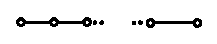
\includegraphics{figures/fig1.eps} & $SL_{n+1}$\\[5pt] 
$B_n (n \geq 3)$ & \qquad 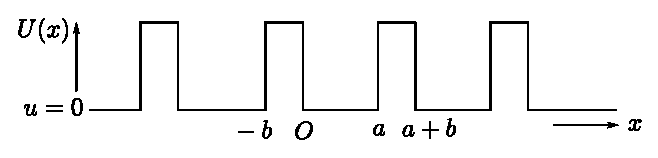
\includegraphics{figures/fig2.eps} & $\Spin_{2n+1}$\\[5pt] 
$C_n (n \geq 2)$ & \qquad 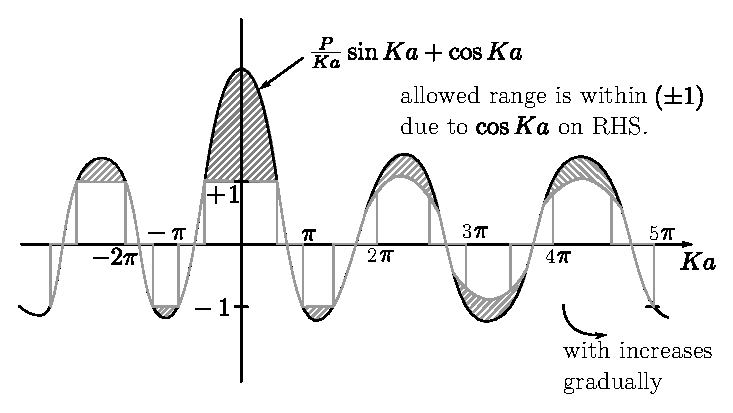
\includegraphics{figures/fig3.eps} & $Sp_{2n}$\\[5pt] 
$D_n (n \geq 4)$ & \qquad 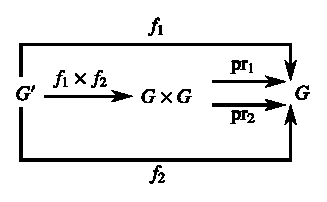
\includegraphics{figures/fig4.eps} & $\Spin_{2n}$\\[5pt] 
$E_6$ & \qquad 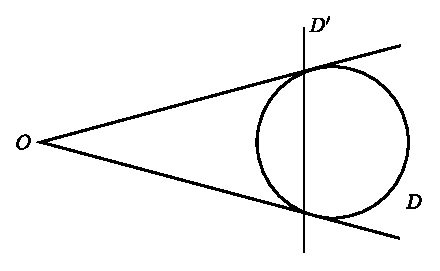
\includegraphics{figures/fig5.eps} & \\[5pt] 
$E_7$ & \qquad 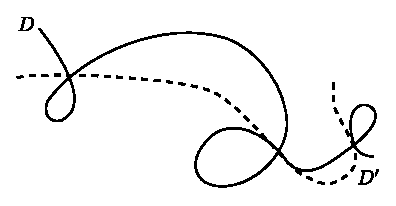
\includegraphics{figures/fig6.eps} & \\[5pt] 
$E_8$ & \qquad 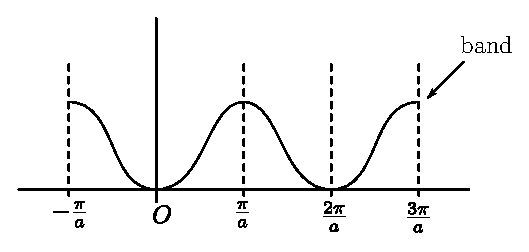
\includegraphics{figures/fig7.eps} & \\[5pt] 
$F_4$ & \qquad 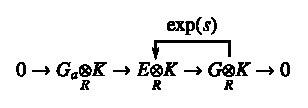
\includegraphics{figures/fig8.eps} & \\[5pt] 
$G_2$ & \qquad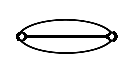
\includegraphics{figures/fig9.eps} & 
  \end{tabular}\pageoriginale
\end{center}

Two simply connected almost simple groups over an algebraically closed
field are isomorphic if and only if they have isomorphic Dynkin
diagrams. The simply connected groups of types $A_n$, $B_n$, $C_n$, $D_n$
are given in the last column; for types $B_n$ and $D_n$ the
corresponding quadra\-tic from must have maximal index. The spin groups
of dimensions 3 to 6 and $Sp_2$ which are not contained in this
list are semisimple too and have the following Dynkin diagrams:    

\begin{center}
\begin{tabbing}
\; $\text{Spin}_3$ \=  \qquad 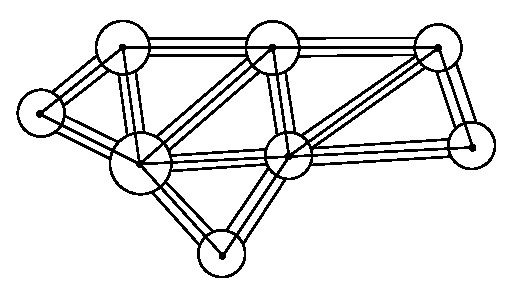
\includegraphics{figures/fig10.eps}\\[5pt] 
\; $\text{Spin}_4$ \> \qquad 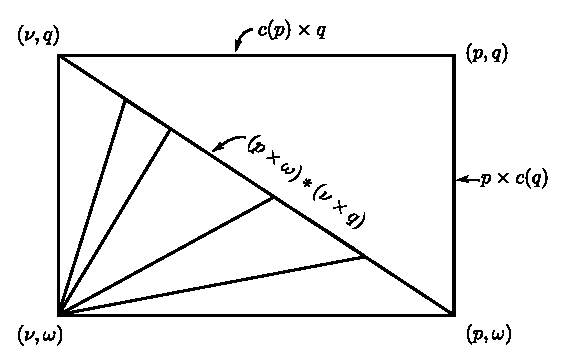
\includegraphics{figures/fig11.eps}\\[5pt] 
\; $\text{Spin}_5$ \> \qquad 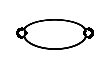
\includegraphics{figures/fig12.eps}\\[5pt] 
\; $\text{Spin}_6$ \> \qquad 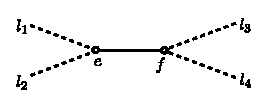
\includegraphics{figures/fig13.eps}\\[5pt] 
\; $Sp_2$ \>  \qquad 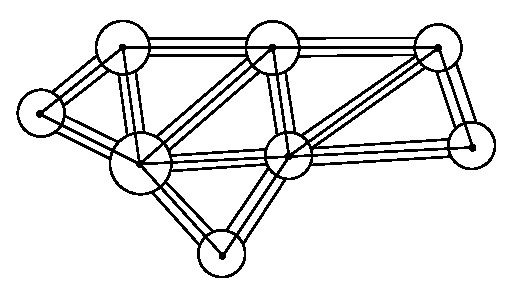
\includegraphics{figures/fig10.eps}
\end{tabbing}\pageoriginale
\end{center}

Looking for isomorphic Dynkin diagrams in our list, we get the
following well known isomorphisms which can otherwise also be proved
without using Dynkin diagrams. (cf. \cite{keyDi}):  

$ \Spin_3  \cong Sp_2 \cong SL_2$ \\

$\Spin_4  \cong Sp_2 \times SL_2$ \\

$ \Spin_5  \cong Sp_4 $ \\

$\Spin_6  \cong SL_4$. \\

It is known that over an arbitrary ground field corresponding to any
of the above types there exists a simply connected group defined over
$K$, having a maximal torus that is defined and split over $K$, it is
unique upto $K$-isomorphism and is called the simply connected
Chevalley group of that  type (cf. \cite{keyC2}, \cite{keyD-G}).   

 The group\pageoriginale Aut $G$ of automorphisms of a simply
 connected group $G$ can 
 also be read off from the Dynkin diagram. It contains the normal
 subgroup of inner automorphisms which is isomorphic to the adjoint
 group $Ad$ $G$, the quotient being the group Symm $(G)$ of
 symmetries of the Dynkin diagram. For Chevalley groups $G$ the Galois
 group $g_{_{\bar{K}/K}}$ acts trivially on Symm $(G)$ and the exact
 sequence  
\begin{equation*}
1 \longrightarrow Ad~ G \longrightarrow Aut~ G \longrightarrow Symm~
(G) \longrightarrow ~1 \tag*{($\ast$)}\label{c2:eqast}
\end{equation*}
splits over $K$. Hence the corresponding cohomology sequence gives a
surjection $ H^1 (K, \text{ Aut } G) \longrightarrow H^1 (K, Symm
(G)) \longrightarrow 1$. Let $G'$ be any $K$-form of a Chevalley group
$G$ belonging to type $X_y$; it determines an element of  $H^1 (K,
\text{Aut} G)$ and taking its image in  $H^1 (K, Symm (G))$ under the
map constructed above we get an element of $H^1 (K, Symm (G)$ say
$a$. Since $ g_{_{\bar{K}/K}}$ acts trivially on Symm $(G)$ a is a
homomorphism of $g_{_{\bar{K}/K}}$ into Symm $(G)$; let $L$ be the
fixed field of the kernel of the homomorphism $a
:g_{_{\bar{K}/K}}\longrightarrow Symm (G)$. Since  Symm $(G)$ is
finite $[L :K ] < \infty$. Let $z =  [L :K ]$. We then say that $G'$
belongs to the sub type ${}^z X_{Y}$. We are now in a position to
define classical groups.  

\begin{defi*}
An absolutely almost simple simply connected group is side  to be a
classical group if it belongs to one of the types  $A_n$, $B_n$, $C_n$,
$D_n$ but not to the subtypes ${}^3 D_4$ and  ${}^6 D_4$. A connected
semi-simple group is called a classical group if in the product
decomposition described above of the simply connected covering group
[cf. this Chapter \ref{chap2:sec2.2}] only classical groups occur
as components.  
\end{defi*}

 We then\pageoriginale see that the simply connected almost simple
 classical grou\-ps 
 defined over $K$ are $K$-forms of $SL_{n+1}$, $Sp_{2n} $ and $\Spin_n$
 (except for some $K$-forms of $\Spin_8$) here $\Spin_n$  corresponds to
 the Spin group of a non-degenerate quadratic form of maximal Witt
 index.  
 

 \section {Classical Groups}\label{chap2:sec2.4}
 
 Following Weil \cite{keyW2} we can describe the simply connected almost
 simple classical groups over $K$ in terms of algebras with
 involution, $K$ being an arbitrary  ground field. Let $G$ be a $K$-form
 of $SL_{n+1}$ belonging to the subtype ${}^1 A_n$  and let $f :
 SL_{n+1} \longrightarrow G$ be the corresponding isomorphism defined
 over $\bar{K}$.  Then for any  $s \in g_{_{\bar{K}/K}}$, $a_s = f^{-1} \circ
 {}^s f \in  \text{Aut} GL _{n+1}$; since $G$ is of subtype  ${}^1 A_n$
 the exact sequence \ref{c2:eqast} of \ref{chap2:sec2.3} shows that
 $a_3$ actually belongs 
 to the adjoint group of $SL_{n+1}$ namely the projectives linear
 group $PGL _{n+1}$ [cf. \ref{chap2:sec2.2} example
   \ref{chap2:exam1}] $(a_s)$ is a 1-cocycle of 
 $g_{_{\bar{K}/K}}$ in  $PGL_n$. Now $PGL_n$ is also the automorphism
 group of $M_{n+1}$, the full matrix ring. Hence $(a_s) \in H^1 (K,
 \text{ Aut } (M_{n+1}))$. Twisting  $M_{n+1}$  by the 1-cocycle
 $(a_s)$ we get a central simple $K$-algebra $A$ and an isomorphism $g :
 M_{n+1} \otimes \bar{K} \longrightarrow A \otimes \bar{K}$ such
 that $a_s = g^{-1} \circ s_g$. Let $H$ be the image of $SL _{n+1}$ under
 $g$. $H$ is an algebraic group defined over $K$. By the definition of
 the reduced norm $N$ in $A$, $N (g(X)) = \det X$, hence $H_{\bar{K}}
 =\bigg\{ x \in  A_{\bar{K}} \bigg/  NX = 1 \bigg\}$. Hence $H$ is
 the algebraic group $\bigg\{ x \in  A \bigg / NX = 1 \bigg\}$. On
 the other hand by means of $g$, $H$ is obtained from $SL_{n+1}$ by
 twisting with the 1-cocycle $(a_s)$ so that $H$ is isomorphic to
 $G$. Hence the $K$-forms of $SL_{n+1}$ belonging to subtype
 ${}^1 A_n$ are the algebraic groups of elements of reduced norm 1
 in central simple $K$-algebras.  
 
 Next\pageoriginale we consider then case when the $K$-from $G$ of
 $SL_{n+1}$ belongs to the subtype ${}^2 A_n$. We can describe $G$
 by means of algebras with involution.   
 
 \begin{defi*}%def 
An antiautomorphism of period 2 of an associative $K$-alge\-bra is
called an involution. An involution is said to be of the first kind if
it fixes every element of the center of the algebra, otherwise it is
said to be of the second kind. An algebra A with involution $I$ is
denoted  by $(A, I)$. In what follows algebras A will be assumed
finite dimensional over $K$. We shall prove that the $K$-forms $G$ of
$SL_{n+1}$ belonging to subtype ${}^2 A_n$ correspond bijectively
with isomorphism classes of simple $K$-algebras $A$ with involution
$I$ of the second kind such that the center is a quadratic extension
of $K$; if $G$ corresponds to $(A,I)$ then $G$ is isomorphic to the
$K$-group $\bigg\{ z \in A \bigg / zz^I = 1, Nz = 1 \bigg\}$. Consider
the algebra $M_{n+1} \otimes M_{n+1}$; this has an involution $I$ of
the second kind given by $(X,Y) \to (^tY,  {}^tX)$ ($t$ denotes
transpose). We shall denote the image of any element  $z \in M_{n+1}
\otimes M_{n+1}$ under $I$ by $z^\ast$. We shall determine all the
automorphisms of $M_{n+1} \oplus M_{n+1}$ 
which commute with $I$; now the automorphism  group of $M_{n+1}
\otimes M_{n+1}$ is generated by inner automorphisms and by the
automorphism $(X,Y) \longrightarrow (Y,X)$ of which the latter
obviously commutes with $I$. If the inner automorphism by the element
a commutes with $I$ it is easy to check that $ a a^I$ must be in the
center $ K \oplus K$ of $M_{n+1} (K) \otimes M_{n+1} (K)$; since
$a a^I$ is invariant under $I$ its components in $K \oplus K$ must be
equal so that $a a^I$ is an element of $K.1$  
  \end{defi*}
   
  If $K$\pageoriginale is algebraically closed we can assume we can
  without loss of 
  generality that $aa^I = 1$, the identity element of $K \oplus
  K$. Hence the group of automorphisms of $M_{n+1} \oplus M_{n+1}$ 
  commuting with $I$ is generated by automorphisms of the types: $1)$
  the automorphisms $(X,Y) \longrightarrow (Y,X)$  $ii)$ inner
  automorphisms by elements of the type $X, {}^t X^{-1}$. Now it is
  well know \cite{keyDi} that the automorphism  group of $SL_{n+1}$ is
  generated by inner automorphisms and by the automorphism $X
  \longrightarrow ^t X^{-1}$ . Hence the imbedding $SL_{n+1}
  \longrightarrow M_{n+1} \oplus M_{n+1}$ given by $X \longrightarrow
  (X, ^t X^{-1})$ gives an isomorphism of the automorphism group of
  $SL_{n+1}$ with the group of those automorphisms of $M_{n+1} \oplus
  M_{n+1}$ commuting with the involution $I$. We shall denote the
  latter group by Aut $(M_{n+1} \oplus M_{n+1},I)$. Let $G$ be a
  $K$-form of $SL_{n+1}$ of subtype ${}^2 A_n$. Then there exists an
  isomorphism $f : SL_{n+1} \longrightarrow G$ over $\bar{K}$ and if
  $s \in g_{_{\bar{K} /K}}$, $a_s = f^{-1} \circ{}^s f $ is a 1-cocycle of
  $g_{_{\bar{K} /K}}$ in $(\text{Aut } SL_{n+1})_{\bar{K}}$ ; but we
  have seen that $(\text{Aut } SL_{n+1})_{\bar{K}} = \text{Aut }
  (M_{n+1} (\bar{K}) \oplus M_{n+1} (\bar{K}), I$. Hence $(a_s)$ is a
  1-cocycle of  $g_{_{\bar{K} /K}}$ in Aut $(M_{n+1} (\bar{K})
  \oplus M_{n+1} (\bar{K}), I$ so that we can twist $M_{n+1} \oplus
  M_{n+1}$ by the cocycle $(a_s)$; the twisted algebra A will carry an
  involution $J$ of the second kind; in this process the center $K
  \oplus K$ of $M_{n+1} \oplus M_{n+1}$ will get twisted into
  the center of $A$; now Symm $(SL_{n+1}) = Z_2$ and since $G$ is of
  type ${}^2 A_n$ the homomorphism $s \longrightarrow \lambda (a_s)$
  of $g_{\bar{K}/K}$ into Symm $(SL_{n+1}) = Z_2$ is non-trivial
  where $\lambda$ is the homomorphism $\lambda : \text{Aut} (SL_{n+1})
  \longrightarrow Symm(SL_{n+1})$ appearing\pageoriginale in the split
 sequence.  
$$
1 \to Ad (SL_{n+1}) \to Aut (SL_{n+1}) \to Symn (SL_{n+1}) \to 1
$$.

 Hence  by \ref{chap1:sec1.7} example \ref{chap1:exam2} Chapter
 \ref{chap1} we conclude that the centre 
$K \oplus K$ of $M_{n+1} \oplus M_{n+1}$  gets twisted into a
quadratic extension $L$ of $K$. Hence $A$ is a simple $K$-algebra with
involution $J$ of the second kind with center a quadratic extension
$L$ of $K$. Now the image of $SL_{n+1}$ under the imbedding $\varphi
:SL_{n+1} \longrightarrow M_{n+1} \oplus M_{n+1}$ constructed above
is given by $\bigg\{ z \in  M_{n+1} \oplus M_{n+1} \bigg/   z z^I=1, Nz
= 1\bigg\} $; the image of this group under the isomorphism $g:
M_{n+1} \oplus M_{n+1} \longrightarrow A $ got by the twisting
process is $\bigg\{ z \in A \bigg / zz^J = 1, Nz = 1\bigg\}$. Hence
taking into consideration the various identifications constructed
above we see that $G$ is isomorphic to the algebraic group $\bigg\{ z
\in A \bigg / zz^J = 1, Nz = 1\bigg\}$ where $A$ is a simple $K$-algebra
with an involution of the second kind with center a quadratic
extension of $K$. 
  
  Next we shall consider the $K$-forms of the Chevally group of
  type $C_n$. Hence the Chevalley group is the symplectic group
  $Sp_{2n} =\bigg\{ X \in M_{2n} \bigg /X S^t X = S \bigg\}$  where
  $S$ is a non-degenerate skew-symmetric matrix over $K$. We shall
  show that the $K$-forms of $Sp_{2n}$ are given by $\bigg\{ x \in A
  \bigg/ xx^J  =1 \bigg\}$  where $A$ is an algebra with involution
  of the first kind $J$, simple with center $K$ and which becomes
  isomorphic to $(M_{2n},I)$ over $\bar{K}$, $I$ being the involution $X
  \longrightarrow S^t X S^{-1}$. The automorphisms of $M_{2n}$
  are all inner automorphisms and the inner automorphism $X
  \longrightarrow u X u^{-1}$ commutes with $I$ and only if $uu^I \in
  K$ above, and again over $\bar{K}$ we may assume $uu^I = 1$, which
  means that $u \in Sp_{2n}$. 
  
  On the\pageoriginale other hand it is known that the only automorphisms of
  $Sp_{2n}$ are inner automorphisms; hence Aut $Sp_{2n}$ Aut $(M_{2n},
  I)$. We can then apply the foregoing method to characterise the
  $K$-forms of $Sp_{2n}$, the result being as indicated in the beginning
  of this paragraph.  
  
  Finally  we shall consider the $K$-forms of Chevalley groups of types
  $B$ and $D$. Here the Chevalley group is $\Spin_n (\mathscr{G}); n$
  may be even or odd $n \neq 1, 2, 3, 4, 5, 6$; and $\mathscr{G}$ is
  a non-degenerate quadratic form of maximal index. Now any
  automorphism of $SO (\mathscr{G})$ is obtained as transformation
  by an element of $O (\mathscr{G})$ i.e. there exists $t \in O
  (\mathscr{G})$ such that $x \to txt^{-1}$ is the automorphism in
  question; but we have seen that any $t \in O (\mathscr{G})$ gives an
  automorphism of the Clifford algebra of $(\mathscr{G})$ (cf. \ref{chap2:sec2.2})
  and so an automorphism of the spin group. All the automorphisms of
  $\Spin (\mathscr{G})$ are obtained in this way through automorphisms
  of $SO (\mathscr{G})$ except in case $D_4$ i.e. $\Spin_8$. This is
  seen as follows: it is clear that the mapping $\tau : \text{ Aut } (SO)
  \to \text{ Aut } (\Spin)$ constructed above is injective; we
  have seen in \ref{chap2:sec2.2} that an inner automorphism of Spin
  $(\mathscr{G})$ by an element $t$ corresponds to an element $u$ of
  $SC$ and by construction $\tau(\text{int } u)$ = int $t$ so that $\tau$
  induces an isomorphism of $Ad(SO)$ onto $Ad (\Spin)$; the index of $Ad
  (\Spin) in \text{ Aut }(\Spin)$ is  equal to the number of
  symmetries of the 
  Dynkin  diagram of the Spin group which is equal to 1 if the
  dimension is odd; if $n$ is even $\neq 8$, the number of symmetries
  is 2, but also the index of $AD (SO)$ in Aut $(SO) = Ad (O)$ is
  2 because transformation by a reflection is not an inner
  automorphism of $SO$. Hence $\tau$ is a bijection in these cases.  
  

  This\pageoriginale shows that the simply connected almost simple
  classical groups 
  of type $B$ and $D$ are two fold coverings of the $K$-forms of the
  special orthogonal group except when the dimension =8 i.e. in the
  case $D_4$. For type $D_4$, every two fold covering of an orthogonal
  group $SO_8$ is easily seen to be of type ${}^1 D_4$ or
  ${}^2 D_4$. Conversely, in the homomorphism of $g_{_{\bar{K}/K}}$
  into Symm $G$ obtained from the twisting cocycle of a group of type
  $D_4$ has image of order 1 or 2 this image can be transformed by
  an inner automorphism into the group of automorphisms induced by $O
  (\mathscr{G})$, and therefore these $K$-forms are coverings of $K$-forms
  of $SO (\mathscr{G})$. Hence classical groups of dimension 8 which
  are $K$-forms of $\Spin_8$ are two-fold coverings of the $K$-forms of
  $SO_8$. Hence in all cases we find that the classical groups which
  are $K$-forms of Chevalley groups of type $B$ and $D$ are two fold
  coverings of the $K$-forms of the special orthogonal group. So we
  have only to find the $K$-forms of $SO (\mathscr{G})$. Let a be the
  matrix of the quadratic from $(\mathscr{G})$ in some basis; on
  $M_n$ define the involution $I$ by $X^I = a^t Xa^{-1}$, $a \in
  M_n$. Using the fact that the automorphisms of $M_n$ are all inner
  we can prove as before that the only automorphisms of $M_n$
  commuting with $I$ are inner automorphisms by elements of
  $0(\mathscr{G})$. Moreover one knows that the automorphisms of $SO$
  are given by transformation by elements of $O (\mathscr{G})$; hence
  over $\bar{K}$ we have an isomorphism Aut $SO (\mathscr{G}) \cong
  \text{ Aut } (M_n, I)$. Carrying out exactly the same procedure as
  before it is easily seen that the $K$-forms of $SO (\mathscr{G})$ are
  given by $G =\bigg\{ x \in A \bigg /xx^J = 1, Nx = 1 \bigg\}$ where
  $A$ is a simple $K$-algebra with involution $J$ of the first kind
  which becomes isomorphic over $\bar{K}$ to $(M_n,I)$. Hence we have
 proved that\pageoriginale simply connected almost simple classical
 groups of types $B$  and $D$ are two fold coverings of groups $G$ 
 given above. 
  

\section{Algebras with involution (cf. [1] Chap
  X)}\label{chap2:sec2.5} 
  
Let $A$ be a simple $K$-algebra with center $L$; let $I$ be an
involution on $A$. If $J$ is another involution on $A$ coinciding with
$I$ on $L$ then by the theorem of Skolem-Noether we can find an
invertible element $a \in A$ such that $x^J = ax^I a^{-1}$ holds for
every $x \in A$. Now, $x = x^{JJ} = a (ax^I a^{-1})^I a^{-1} =
(aa^{-I}). x (aa^{-I})^{-1}$ for every $x \in A$, so that $aa^{-1} \in
L$. Let $a^{I}=ca$ where $c \in L$; applying $I$ to both sides we get
$cc^I = 1$. If the involution is of the first kind (See
\ref{chap2:sec2.4} for the 
definition) $cc^I = 1$ implies $c^2 = 1$ i.e. $c = \pm 1$ so that $a^I =
\pm a $. Suppose now that $I$ is of the second kind, let $F$ be the
fixed field of $I$ in $A$; then since $I$ is of period 2, $L$ is a
quadratic extension of $F$ and the condition $cc^I = 1$ is equivalent
to $N_{L/F} (c) = 1$. Hence by Hilbert's theorem 90, there exists
$d \in L^*$ such that $c = d^I d^{-1}$. Therefore $a^I = ca = d^I
d^{-1}a$, i.e $(d^{-1}a)^I = d^{-1} a$. Moreover the equation $x^J =
ax^I a^{-1}$ is unaltered if we replace a by $d^{-1}a$ since $d \in
L$. Hence if $I$ is of the second kind we can assume in the equation
$x^J = ax^I a^{-1}$ that $a^I = a$. 

  
\medskip
\noindent\textbf{Examples of algebras with involution:}
  A quaternion algebra with the standard involution $x \to \bar{x}$,
  the conjugate of $x$, is a simple algebra and the standard
  involution is of the first kind. If $D$ is any division algebra
  over $K$ then $M_n(D)$ has an involution of the $r^{\rm th}$ kind $(r =
  1,2)$ if and only if $D$ has an involution of the $r^{\rm th}$ kind; for
  if $I$ in an involution\pageoriginale of the rth kind on $D$ then if
  we define 
  $X^J$ for $X = (x_{ij}) \in M_n (D) $ as $X^J = (x^I_{ji})$  we get
  an involution of the $r^{\rm th}$ kind; the converse follows from Theorem 1
  below by taking $A = M_n(D)$, $B = M_n (K)$. 
  
  Next let $A$ be a simple $K$-algebra with an involution $I$; let $L$ be
  the center of $A$. Suppose $B$ is a given $K$-subalgebra of $A$
  containing $L$ and assume moreover that $B$ carries an involution
  $J$ coinciding with $I$ on $L$. When can $J$ be extended to an
  involution on $A$? Sufficient conditions under which this is
  possible are given by the following     

\begin{theorem*}
With the notations as above $J$ can be extended to an involution on
$A$ in the following cases: 
  \begin{enumerate}[i)]
\item  $B$ is a simple algebra

\item $B$ is a maximal commutative semi-simple subalgebra of $A$ and 
  $I$ is of the second kind. 
\end{enumerate}
\end{theorem*}

\begin{proof}
$I~ o~ J$ is an isomorphism of the $L$-algebra $B$ into the simple
  algebra $A$ with center $L$ so that in case $i)$ by the theorem of
  Skolem-Noether we can find an invertible element $t \in A$ such that
  $x^{IoJ} = (x^J)^I = txt^{-1}$ for every $x \in B$; this conclusion
  holds true also when $B$ is a maximal commutative semi-simple
  subalgebra of $A$ \cite{keyK1} Hilfssatz 3.5. Let
  $B'$ be the commutant 
  of $B$ in $A$; let $L(u)$ be the $K$-subalgebra generated  by $u =
  t^{-I} t$. If $v$ is any element of $B'$ and if we replace $t$ by
  $tv$ in $x^J = (txt^{-1})^I x \in B$ found above this equality is
  unaltered; we shall choose a suitable $v \in B'$\pageoriginale and
  replace $t$ by 
  $tv$ in the final stage to obtain an involution extending $J$; for
  the moment let $u= t^{-I}t$ with $t$ as given above. Define for
  every $x \in A$, $x^{\widetilde{J}} = (\text{txt} ^{-1})^I $;  then
  by what precedes ${\widetilde{J}}$ coincides with $J$ on $B$;
  moreover if $x \in B$, $x^{{\widetilde{J}}^2}= (tx^Jt^{-1})^I =
  t^{-I} \cdot (x^J)^I \cdot t^I = t^{-I} (txt^{-1}) \cdot t^I =  
  uxu^{-1}$; but $x^{{\widetilde{J}}^2} = x^{J^{2}}= x$ since $x \in
  B$ so that $uxu^{-1}=x$ implying that $u \in B'$ and hence
  $L(u)\subset B'$. It 
  will turn  out the we can choose $v \in L(u)$ suitably so that when
  $t$ is replaced by $tv$, and $\widetilde{J}$ defined as
  above  with this new $t$  then $\widetilde{J}$  will be an
  involution on $A$, extending $J$ on $B$. The equation $x^{\widetilde{J}^2}
  = uxu^{-1}$ shows that if we choose $v \in B'$ to satisfy
  $(tv)^{-I}(tv)=\pm 1$ then with $tv$ in place of $t$ the equation
  $x^{\widetilde{J}^2}=x$ will hold for all $x \in A$ and consequently
  $\widetilde{J}$ will be an involution on A; evidently
  $\widetilde{J}$ will then 
  be an extension of $J$ on $B$. We shall prove that $ v \in L(u)$ can
  be chosen so as to satisfy $(tv)^{-I}(tv) = \pm 1$. Observe that  
$$
u^{\widetilde{J}}u = (tut^{-1})^I. u =(t^{-I}. u^I . t^I). (t^{-I}.t)
= t^{-I}u^I.t  =t^{-I}.t^I.t^{-I}.t =1
$$
hence $u^{\widetilde{J}}=u^{-1}$. Consider case $i)$ first. If $u=-1$,
then  evidently the 
choice $v =1$ will do, so assume $u \neq -1$. To start with assume
$B'$ to be a division algebra; the condition $(tv)^{-I}tv =1$, is
equivalent to $v^{-\widetilde{J}} u v =1$; we claim that
$v=(1+u)^{-1}$ which is obviously an element of $L(u)$ will work; for
$v^{-\widetilde{J}}=1+u^{\widetilde{J}} = 1+u^{-1}= (1+u) \cdot u^{-1}
= v^{-1}.u^{-1}$ so
that $v^{-\widetilde{J}}  uv =1$. Suppose now $B'$ is not
necessarily a division algebra, we can write $B' \cong D
\otimes M_n$ where $M_n$ is the full matrix ring of dimension $n^2$
for some $n$ 
and $D$ is a division algebra. We can\pageoriginale then consider $D$,
$M_n$ as 
subalgebras of $A$; the commutant of the subalgebra $BM_n$ is equal
to the commutant of $M_n$ is $B'$, i.e. to $D$. Now the involution $J$
on $B$ can be extended to $BM_N$ by defining $(bX)^{J'} = b^J {}^t X$, $b
\in B$, $X \in M_n$. Moreover $BM_n$ is a simple algebra being
$L$-isomorphic to $B \otimes_L M_n$ which is simple. Hence by the case
already considered the involution $J'$ can be extended to an
involution of $A$; this extension clearly coincides with $J$ on $B$. 

Next consider case $ii$). Here again we shall find $v \in L (u)$ to
satisfy $(tv)^{-I}(tv) = 1$  i.e. $v^{-\widetilde{J}}uv=1$.  Since
$u^{\widetilde{J}}= u^{-1}$, $\widetilde{J}$ maps $L(u)$ onto itself;
it is an involution of $L(u)$ of the second kind. Let $F$ be the fixed
field of $\widetilde{J}$ in $L$. Let $C^+$ be the subalgebra of
elements of $L(u)$ fixed by $\widetilde{J}$;  since $\widetilde{J}$ is
not the identity on $L$, $L(u) \cong C^+ \oplus_F L$; moreover under
this isomorphism the action of $\widetilde{J}$ on $L(u)$ goes over into the
natural action of the Galosi group $g_{L/F}$ of $L/F$ on $C+ \otimes_F
L$. The elements of $g_{L/F}$ are 1 and $\tilde{J}$; the
correspondence
$\overset{\sim}J \to u^{-1}$, $1 \to 1$ defines a 1-cocycle of $g_{L/F}$
in $(C^+ \otimes_F L)^*$. By \ref{chap1:sec1.7} Chapter \ref{chap1}
we know that $H^1
(L/K,(C^+)^*) =1$; hence there exists $v \in L(u)$ such that
$v^{-1}u^{-1}v^{\widetilde{J}}=1$, i.e. $v^{-\widetilde{J}} uv
=1$. But this is what we wanted. Hence the theorem is completely
proved. 

If $A$ is a central simple algebra over $K$ and if $A$ has an
involution $I$ of the first kind then $A$ is of order 1 or 2 in
the Brauer group of $K$; for $I$ gives an isomorphism of $A$ with its
opposite algebra $A^o$ hence $A \otimes_k A \cong A \otimes_k
A^0$ splits. But if $I$ is of the second\pageoriginale kind $A$ is not
necessarily isomorphic over the centre to its opposite algebra, so
may not have order 2 in the Brauer group (for an example see \S
\ref{chap5:sec5.1}). But let us consider the particular case where $A$ is a
quaternion algebra with centre $L$ and assume that $I$ is an
involution of the second kind. Let $K$ be the subfield of $L$ fixed by
$I$ so that $L$ is a quadratic extension of $K$. Let $J$ be the
standard involution on $A$ namely conjugation; this is the only
involution on $A$ which fixes exactly the elements of $L$. The
involution $IJI^{-1}$ fixes the centre so that $IJI^{-1}= J$, 
i.e. $(IJ)^2=$ identity. Let $B$ be the fixed space of $IJ$ in $A$; then
$B$ is a $K$-subalgebra of $A$, and $A \cong B \otimes_K L$
since $IJ$ is not the identity $L$. Hence we have proved the following  
\end{proof}

\setcounter{proposition}{0}
\begin{proposition}\label{chap2:prop1}%%% 1
 If $A$ is a quaternion algebra of centre $L$ and has an involution
 $I$ of the second kind then $A \cong B \otimes_K L$ where $B$ is an algebra
 over the fixed field $K$ of $I$. Moreover $I$ coincides with the
 standard involution on $B$ and on $L$ it coincides with the
 non-trivial $K$-automorphism. 
 \end{proposition}
 

 \section{Bilinear and hermitian forms; discriminants}\label{chap2:sec2.6}
 
 Let $D$ be a division algebra; let $x \rightarrow \bar{x}$ be an
 involution; let $V$ be a $n$-dimensional left vector space over
 $D$. A sesquilinear form on $V$ is a function $B:V \times V
 \rightarrow D$  taking $(x,y)$ to $B(x,y)$ which is linear in $x$ and
 anti linear in $y$ (i.e. $B(x,\alpha y)=B(x,y) \bar{\alpha}$ for every
 $x,y \in V, \alpha \in D$), $B$ is called hermitian if we have
 $B(x,y)=\overline{B(y,x)}$ for every pair of vectors $x,y \in V$; $B$
 is called skew\pageoriginale hermitian if $B(x,y)=
 -\overline{B(y,x)}$ for every 
 pair of vectors  $x,y \in V$. Let $h(x) =B(x,x)$; we shall call $h$ a
 hermitian or skew hermitian form according as $B$ is a hermitian or
 skew-hermitian sesquilinear form. If $e_1,\ldots, e_n$ is a $D$-basis of
 $V$, then the matrix $(B(e_i,e_j))$ is said to be the matrix of $B$
 relative to this basis. Call this matrix $M$. If $e'_1, \ldots,e'_n$
 is any other basis of $V$ let $e'_i = \sum\limits_{i=1}^{n}
 \alpha_{ji}e_i$ and denote the matrix $(\alpha_{ij})$  by the
 letter $T$; then the matrix of $B$ in the basis $e'_1 , \ldots,e'_n$
 is just ${}^t TM \bar{T}$. We define the radical of $V$ as the space
 of elements $x \in V$ such  that $B(x,y)=0$ for every $y \in V$. $B$
 is said to be non-degenerate if the radical is zero. Any hermitian
 space $V$ has an orthogonal basis i.e. a basis $e_1,\ldots, e_n$ such
 that $B(e_i,e_j)=0$  if $i \neq j$; for $e_1$ one can choose any
 anisotropic vector i.e such that $B(e_1,e_1) \neq 0$. If $V,V'$ are
 two hermitian spaces over $D$ withe corresponding hermitian form
 $B$, $B'$ then a $D$-linear transformation $\sigma :V \rightarrow V'$ is
 called an isometry if $\sigma$ is bijective and $B(x,y)=B(\sigma
 x,\sigma y)$ for every  $x,y \in V$. In particular if $V=V'$ the set
 of isometries of $V$ onto itself will be a group called the unitary
 group of the hermitian form. 
 We have similar notions for skew-hermitian forms over $D$.
 
 Let $V$ be a finite dimensional vector space over $K$ endowed with a
 quadratic form $\mathscr{G}$ which we assume to be
 non-degenerate. The determinant of the matrix of $(V, \mathscr{G})$
 with respect to any basis of $V/K$ is unique modulo squares of $K^*$,
 i.e. it is a well defined element of $K^*/K^{*2}$. We call this
 element of $K^*/K^{*2}$ the discriminant of $V$.\pageoriginale Quite
 frequently a 
 representative in $K^*$ will be called the discriminant of $V$; this
 will not involve any confusion as the context will make it clear what
 we have in mind. Let $D$ be a quaternion division algebra over $K$
 with the standard involution; let $V$ be a finite dimensional left
 vector space over $D$. If $h$ is a hermitian of skew hermitian form
 on $V$ the discriminant of $h$ is by definition the reduced norm of
 a matrix representing $h$, modulo squares of elements of $K^*$. We
 shall state and prove a number of lemmas which we shall need in the
 sequel. 

\setcounter{lem}{0}
  \begin{lem}\label{chap2:lem1}%lemma 1a
a) ~ Let $D$ be a quaternion algebra over $K$; let $h$ be a
non-degenerate hermitian or skew hermitian form on a finite
dimensional vector space $V$ of $D$. Then if $D$ does not split, the
special unitary  group $SU(h,D)$ of $h$ coincides with the unitary
group $U(h,D)$. More generally we shall prove the following  
 \end{lem} 
 
\setcounter{lem}{0}
 \begin{lem}%lemma 1b
b) ~ Let $A$ be a simple central $K$-algebra with an involution $I$ of the
first kind. If there exists an element $x\in A$ satisfying $xx^I =1$
and $Nx=-1$, then $A \cong M_n(K)$.        
 \end{lem} 
 
\begin{proof}
We look at the eigen values of $x$ considered as an element of $A
\otimes_K\bar{K} \cong M_n(\bar{K})$. Since every involution
of $M_n(\bar{K})$ is transposition followed by an inner automorphism,
$x$ and $x^I$ have the same eigenvalues. But $x^I = x^{-1}$, so $x$
and  $x^{-1}$  have the same set of eigenvalues and with equal
multiplicities. This implies that the eigenvalues of $x$ different from
$\pm 1$ occur in pairs $(\lambda, \lambda^{-1})$. Since the product of
the eigenvalues is equal to the reduced norm of $x$, $-1$ must occur as
eigenvalue with odd multiplicity. 
\end{proof}

\noindent
This\pageoriginale shows that 0 is an eigen value of $x+e$ ($e$
denoting the identity of $A$) of odd multiplicity. Hence if the 
integer $m$ is sufficiently large the null space of $(x+e)^m$ is of
odd dimension.   

Now go back to the ground field $K$. We can write $A \cong M_k
(D)$. Let $n^2 = [A:K]$; we then have $[D:K]=(n/k)^2$. The lemma
will be proved if we show that $[D:K]=1$. For this we compute the
dimension over $K$ of the $K$-space $\Lambda =\{ y \in M_k (D) | (x+e)^m
.y=0\}$, in two different ways and compare them.  

Let $V$ be a $K$-dimensional left vector space over $D$. We can then
interpret $(x+e)^m, y$ as linear transformations on $V$. Then $y \in
\Lambda $ if and only if $y$ maps $V$ into the kernel of
$(x+e)^{m}$. From this description of the elements of $\Lambda $ it is
easy to see that $[ \Lambda  :D]=k.r$, where $r$ denotes the dimension
over $D$ of the kernel of $(x+e)^m$.  Hence $[ \Lambda  :K]=k.r
[D:K]=k.r(n/k)^2=nr (n/k)$. On the other hand
$[\Lambda :K]=[\Lambda_{\bar{K}} : \bar{K}]$. Now $\Lambda_{\bar{K}}$ is equal to
$\left\{y \in M_n (\bar{K})/(x+e)^m y=0 \right\}$ so that by the same
argument as 
above with $D$ replaced by $\bar{K}$ we  get $ [\Lambda_{\bar{K}}:
  \bar{K}]=n (\dim_{\bar{K}} \ker (x+e)^m)$. But by the first part of
the proof $\dim_{\bar{K}} \ker (x+e)^m$  is an odd integer. Hence
$[\Lambda : K]=n x$ an odd integer. Comparing the two values of
$[\Lambda :K]$ obtained we get $nx odd$ integer $=n.r(n/k)$. This
implies $n/k$ is odd integer. i.e. $[D:K]$ is an odd integer. Now $A$
being an algebra  with involution of the first kind it has order two
in the Brauer group. But one knows that the prime divisors of the
order of $A$ in the Brauer group and those of $[D:K]$ are the same. 
The last two conclusions can hold simultaneously only when $[D:K]=1$.

This proves the lemma.

\begin{lem}\label{chap2:lem2}
Let $D$\pageoriginale be a quaternion algebra over $K$ with an involution
$I$, $A=M_n(D)$; for $Z= (z_{ij}) \in A$ denote by $Z^*$ the element 
$(z_{ji}^I)$. Let $a \in A $ be a non-singular skew-hermitian matrix,
i.e. $a^*=-a$. Then if $X,Y$ are $1 \times n$ matrices over $D$ such
that $XaX^* = YaY^*=C$ is non-singular in $D$, there exists a proper
$a$-unitary matrix $t \in A$ such that $Y=Xt$. 
\end{lem}

\begin{proof}
If $D$ is a division algebra, this follows immediately from Witt's
theorem and lemma \ref{chap2:lem1}. If $D= M_2 (K)$, the action of $I$ is as
follows: $\alpha \rightarrow S^t \alpha S^{-1}$ where $S$
is some fixed $2 \times2$  skew-symmetric matrix in $M_2
(K)$. Denoting by $P$ the $2n \times 2n$ matrix  
$\begin{pmatrix}
S & &\\
& S_. &\\
& & ^.S
\end{pmatrix}
$ we have $X^* = P^t XS^{-1}$, $Y^* = p^t YS^{-1}$ and
$a^*=p^tap^{-1}$. Now since $a^* =-a$, we have $p^t ap^{-1} =-a $
which implies that $aP =- P^t a = ^t(ap)$. This shows  that $aP$ is a
symmetric $2n \times 2n$ matrix. The condition $XaX^*=c$ then gives
$X(aP)^tX=cS$; similarly the condition $YaY^*=c$ gives
$Y(aP)^tY=cS$. The matrix $aP$ gives  a $2n \times 2n$ dimensional
quadratic space over $K$ and the above two equations imply that the
two dimensional subspaces generated by the two rows of $X$ and $Y$
respectively are isometric. Hence by Witt's theorem on quadratic form
there exists an isometry $t$  of the above quadratic space
transforming $X$ into $Y$. If $t$ is not proper then by multiplying
$t$ on the right by a reflection in a suitable subspace containing the
two rows of $X$ we can make the product proper. Hence $t$ can be
assumed proper. This $t$ then defines a proper unitary transformation
changing $X$ into $Y$. 
\end{proof}

\begin{lem}\label{chap2:lem3}
Let $D$\pageoriginale be a quaternion division algebra with standard
involution; $(V,h)$ and $(V', h')$ are two skew hermitian spaces  over
$D$. Let $f:(V_{\bar{K}},h) \rightarrow(V'_{\bar{K}},h')$ be an isomorphism
over $\bar{K}$; then the 1-cocycle $a_s=f^{-1} o {}^s f$ which belongs
to $H^1(K,U)$ comes from $H^1(K,SU)$ if and only if the discriminants of
$(V,h)$ and $(V',h')$ are equal; here $U$ denotes the unitary
group and $SU$ denotes the special unitary group of $h$. 
\end{lem} 

\begin{proof}
Consider the exact sequence $1 \rightarrow SU \rightarrow U
\rightarrow Z_2 \rightarrow 1$ where $U \rightarrow Z_2$ is the norm
mapping; this gives rise to an exact sequence $H^1 (SU) \rightarrow
H'(U) \rightarrow H^1(Z_2)$; but clearly $ H^1(Z_2) \cong
K^*/K^{*^2}$ and\break $H^1 (U) \rightarrow K^*/K^{*^2}$ is the map
associating with each $K$-form $(V', h')$ of $(V,h)$ the quotient of
the discriminants of $h'$ and $h$. This shows that $(a_s)$ comes from
$H^1 (SU)$ if and only  if $V'$ has the same discriminant as $V$. 

Next we shall determine the simply connected absolutely almost simple
classical groups of types $B_n$, $C_n$, $D_n$ over fields $K$ satisfying
the property that every division of order 2 in the Brauer group
$B_L$ for any algebraic extension $L$ is a quaternion
algebra. Examples of such fields are the $\mathscr{P}$-adic fields and
number fields \cite{keyDe}. If $A$ is a central simple involutorial algebra
over such a field $K$ then since its order in Brauer group is either
1 or 2 we conclude that either $A$ is a matrix algebra over $K$ or
a matrix ring over a quaternion division algebra over $K$. We make use
of the classification given in \ref{chap2:sec2.4}. Consider $G=\{ x \in A/
xx^I=1\}$ where $A$ is a central simple $K$-algebra with\pageoriginale
involution $I$ of the first kind. There are two possibilities $i) A
\cong M_r (K) $ or $ ii) A \cong M_s(C)$ where $C$ is
a quaternion 
division algebra over $K$. In the first case there exists an
invertible $a \in M_r(K)$ either symmetric of skew-symmetric such
that $X^I =a^t X a^{-1}$ for every $X \in M_r(K)$. If $a$ is
skew-symmetric $G$ is the symplectic group of the alternating form a
and so belongs to type $C_n$; but if a is symmetric we get the
orthogonal group which will correspond to type $B_n$, $D_n$ by taking
two-fold coverings of the special orthogonal group. In the second
case when $A \cong M_s(C)$, $C$ being quaternion division algebra
we get $x^I = ax^* a^{-1}$ where $x \rightarrow x^*$ is the involution
on $M_s (C)$ given by $(x_{ij}) \rightarrow (\bar{x}_{ji})$, denoting
the standard involution on $C$ and where a is either hermitian or skew
hermitian with  respect to $^*$. In the first case $xx^I =1$ means that $x$
is in the unitary group of the hermitian form while in the second case
it means that $x$ is in the unitary group of the skew-hermitian form
$a$. Consideration of the dimension of the space of symmetric elements
will show that the former corresponds to type $C_n$ while the latter
to type $D_n$. Hence we have the  
\end{proof}

\begin{theorem*}%the 
The only simply connected absolutely almost simple Classical groups of
types $B_n$, $C_n$, $D_n$ over a field with the properties stated above
are 

\noindent
$C_n$: Symplectic groups and unitary groups of hermitian forms over
qua\-ternion division algebras 

\noindent
$B_n$, $D_n $: Spin groups of quadratic forms and of skew hermitian
for\-ms over quaternion division algebras. 
\end{theorem*}


